\documentclass[10pt,a4]{article}
\usepackage{fullpage}
\usepackage{graphicx}
\usepackage{hyperref}
\usepackage{longtable}
\usepackage{array}
\usepackage{booktabs} % Required for using \toprule, \midrule, and \bottomrule in tables

\usepackage{calc}  % Add this to handle calculations
\newcommand{\real}[1]{#1}  % Define real if not already defined

\def\tightlist{%
  \setlength{\itemsep}{0pt}\setlength{\parskip}{0pt}}

\title{De-Identification Tool for Clinical Reports}
\author{Marc Zimmermann$^1$, Katie Kalt$^2$, Patrick Hirschi$^2$, and\\
  Gunnar R\"atsch$^{1,2}$\\
{\footnotesize $^1$ Biomedical Informatics Group, Department of Computer Science, ETH Zurich, Zurich, Switzerland}\\
{\footnotesize $^2$ Department Research and Teaching, University Hospital Zurich, Zurich, Switzerland}}
\date{October 2021}

\begin{document}

\maketitle

\begin{abstract}
This document outlines the development and implementation of a robust
software tool designed to de-identify clinical reports to address
privacy regulations and policies. The tool employs advanced natural
language processing techniques to accurately identify and anonymize
personal health information (PHI) from clinical texts, making them
suitable for further research and analysis without compromising
patient confidentiality. Key components of the software include a
customizable annotation pipeline, extensive lexica for precise entity
recognition, and sophisticated algorithms for sensitive data detection
and substitution. The document also details the software's
architecture, setup requirements, usage guidelines, and performance
metrics, supported by a case study on its application in a real-world
healthcare setting. This comprehensive approach not only supports
using the tool to meet regulatory requirements but also adapts
efficiently to varied data formats and clinical environments.
\end{abstract}

\newpage

\tableofcontents
\newpage

\section{Introduction}
%\section{Overview}\label{overview}

The deidentification tool consists of a collection of command line
applications written in Java. The applications is based on the
\href{https://gate.ac.uk/}{GATE framework}

Here, a short overview over each command line application. Each square
box represents a different command described in the following sections.

\begin{figure}
\centering
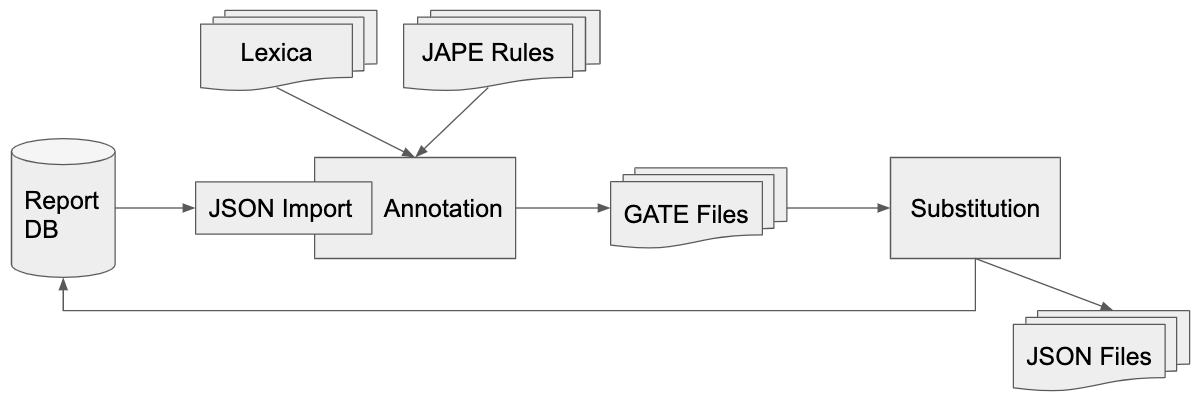
\includegraphics[width=\textwidth]{figs/system_overview.png}
\caption{System overview}
\end{figure}

\subsection{Document Import}\label{document-import}

The deidentifier tool imports JSON reports typically from a database
(json reports on the filesystem are also supported) and converts them to
a GATE compatible representation. The \texttt{annotate} command can read
directly from the appropriate source. The \texttt{import} command only
does the import and conversion step and stores a batch of documents into
a GATE corpus (which is a directory on a filesystem).

It is assumed that the documents are stored in a database table or view,
one row per document. The actual report content is encoded as JSON
string in one of the columns. Other required columns denote the document
type (\texttt{FCODE}) as well as the report id.

The tree like structure of the JSON documents is preserved during the
conversion to the GATE compatible representation. This can be exploited
during the annotation.

\subsection{annotate}\label{annotate}

The \texttt{annotate} command takes documents from a GATE corpus and
runs an annotation pipeline over the reports, i.e.~annotates portions of
the text which contain entities to be deidentified. The output of this
process is again a GATE corpus, which can be examined e.g.~using the
\href{https://gate.ac.uk/download/}{GATE developer tool}.

An \emph{annotation} simply denotes a span of text with some properties
associated, for example: ``Mr.~Muster, born 01.01.1964 in Aarau'' could
have 3 annotations related to deidentification: one for `Muster' (Name),
another for `01.01.1964' (Date, with the additional information that it
is a birthdate) and `Aarau' (Location).

Currently, the following entities are annotated: * Age * Contact
(distinguishing phone numbers, email and websites) * Date (if possible
determining birth date, admission date, discharge date) * ID (patient or
case ID, social security or insurance numbers) * Name (if possible
distinguishing patient from staff) * Location (broad category containing
geographical locations as well as organizations) * Occupation

The annotation pipeline consists basically of the following consecutive
steps:

\begin{figure}
\centering
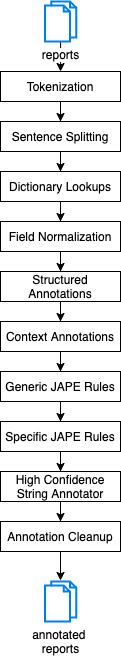
\includegraphics[width=0.2\textwidth]{figs/pipeline_overview.png}
\caption{Pipeline steps}
\end{figure}

\begin{enumerate}
\def\labelenumi{\arabic{enumi}.}
\tightlist
\item
  \textbf{Tokenization}: splitting the text into units of characters
  (`words'), for example `Mr.~Muster' would be split into 3 tokens `Mr',
  `.' and `Muster'
\item
  \textbf{Sentence Splitting}: Grouping tokens together into sentences
\item
  \textbf{Lookups}: Annotating tokens using dictionaries/lexica (called
  ``Gazetteers'' in GATE). For instance, the tokens `Universitätsspital
  Zürich' could be annotated as ``organsation'' and the token ``Zürich''
  as ``location''
\item
  \textbf{Field Normalization}: Renaming some fields in the report to a
  common name to simplify downstream steps. E.g. \texttt{AddrLine},
  \texttt{Address}, \texttt{Adresse} could all be renamed to
  \texttt{AddressField}.
\item
  \textbf{Structured Annotation}: annotate entire fields known to
  contain information to be deidentified. For example, the content of a
  field \texttt{Tel} denoting a phone number could immediately be
  annotated without having to apply any further processing.
\item
  \textbf{Context Annotation}: annotate a window (of tokens) around some
  trigger token with a \href{components.md\#context-annotations}{context
  annotation}. like \texttt{NameContext} or \texttt{OccupationContext}
  to help JAPE rules to disambiguate between e.g.~surnames and
  professions.
\item
  \textbf{JAPE rules}: annotate tokens based on a regular
  expression-like language. This is based on the structure or content of
  tokens (e.g.~a specific trigger word such as ``Dr'' or being a number)
  as well as previous annotations from dictionaries from the previous
  step. Note, that rules can also exploit the tree-like structure of the
  document, for example a rule may only apply if the token in a field is
  part of the section of the document related to patient information.
\item
  \textbf{High Confidence String Annotator}: Some JAPE rules in the
  previous step can be marked as \texttt{high\ confidence}, that is,
  whatever these rules annotate, we have high confidence that it is
  correct. The \texttt{HighConfidenceStringAnnotator} then checks what
  tokens were annotated by a high confidence rule and then annotates the
  same tokens in the remaining document.
\item
  \textbf{Clean up}: resolve overlapping or conflicting annotations
  using heuristics.
\end{enumerate}

\subsubsection{JAPE Example}\label{jape-example}

Here an example of a JAPE rule. We are interested in recognizing ages in
a very specific pattern, namely the age followed by ``jährige'',
``jähriger'' or ``jährigen'', e.g.~``59-jähriger Patient'':

\begin{verbatim}
// 0-119 (including decimals)
Macro: POSSIBLE_AGE
(
    ({Token.string ==~ "[1-9]*[0-9]"} | {Token.string ==~ "1[0-1][0-9]"})
    ({Token.string == "."} {Token.string ==~ "[0-9]+"})?
)


Rule: AgeRightContextTrigger
(
   (POSSIBLE_AGE):age
   ({Token.string == "-"})?
   ({Token.string ==~ "jährige[rn]?"})
)
-->
:age.Age = {rule = "AgeRightContextTrigger"}
\end{verbatim}

Rules describe a sequence of tokens on the ``left hand side'',
i.e.~before ``--\textgreater{}''. If such a sequence is recognized in a
text a rule is triggered and the ``right hand side'' is applied. In the
above case, the right hand side adds an annotation of type \texttt{Age}
having as a property the name of the rule triggered (this helps
debugging).

A token can be described exactly, like
\texttt{\{Token.string\ ==\ "-"\}} where the token should consist
exactly of \texttt{-} or using regular expressions as in
\texttt{\{Token.string\ ==\textasciitilde{}\ "1{[}0-1{]}{[}0-9{]}"\}}
describing the numbers from 100 to 119. A sequence of tokens may contain
optional elements denoted with \texttt{?}. In the above example the
\texttt{(\{Token.string\ ==\ "-"\})?} signifies, that there may or may
not be a dash.

More details regarding JAPE can be found in the
\href{https://gate.ac.uk/sale/thakker-jape-tutorial/GATE\%20JAPE\%20manual.pdf}{JAPE
Grammar Tutorial}

Note, that the above example is not robust against typos, e.g.~the rule
would fail to annotate the age in ``59-järiger Patient''.

\subsection{substitute}\label{substitute}

Takes an annotated GATE corpus and generates a JSON representation of
the content with to be deidentified tokens replaced. The JSON version of
these reports can then be saved back to a database table or to JSON
files on a drive one per report.

\subsubsection{Substitution Policies}\label{substitution-policies}

There are several policies implemented on how annotated tokens should be
replaced:

\begin{itemize}
\tightlist
\item
  \texttt{ScrubberSubstitution}: entities are replaced by a fixed string
  depending on the annotation type, for example `am 01.02.2003' would be
  replaced as ``am DATE'' and `Dr.~Muster' by `Dr.~NAME'
\item
  \texttt{DateShift}: same as \texttt{ScrubberSubstitution}, but all
  dates of a report are shifted by a random amount of days into the
  future or past.
\item
  \texttt{ReplacementTags}: In this policy information are passed along
  to a downstream application which takes care of the actual
  deidentification. For that purpose entities are replaced by `tags'
  which contain as much information as possible from the annotation
  pipeline. For example a text like ``Dr.~P. Muster empfiehlt'' could be
  replaced by
  \texttt{Dr.\ {[}{[}{[}Name;P.\ Muster;firstname=P;lastname=Muster;type=medical\ staff{]}{]}{]}\ empfiehlt}
  that is, the original value is preserved and the downstream
  application can decide how to replace the name most appropriately.
\end{itemize}

There exist also the \texttt{-\/-fields-blacklist} option, where a list
of field names can be provided which are completely erased from the
document. This can be useful for fields with are notoriously hard to
deidentify, but contain no relevant information for a downstream
application.


\section{System Setup and Requirements}
\subsection{Installation}\label{installation}

\subsubsection{Prerequisites}\label{prerequisites}

\begin{itemize}
\tightlist
\item
  at least Java 8
\item
  appropriate JDBC driver, if reports are loaded from database
  (PostgreSQL drivers are already included)
\end{itemize}

\subsubsection{Getting the Software}\label{getting-the-software}

Download the latest release from the
\href{https://github.com/ratschlab/medical-reports-deidentification/releases}{releases
page}, that is, the jar file in the \texttt{Assets} section.

Alternatively (more advanced), you can download a recent zip archive
generated everytime the github action workflows are triggered. You can
look for
\href{https://github.com/ratschlab/medical-reports-deidentification/actions}{workflow
runs of the branch ``main''} and look for the ``Artifacts'' section of a
specific run.

\paragraph{Building Yourself}\label{building-yourself}

You need'll need \href{https://maven.apache.org/install.html}{Maven} to
build from source code. Once \texttt{maven} is set up, you can run the
following in the root directory of the repository

\begin{verbatim}
mvn package --file deidentifier-pipeline/pom.xml
\end{verbatim}

You'll then find the \texttt{jar} file containing the pipeline code as
well as its dependencies in \texttt{deidentifier-pipeline/target}

\subsubsection{Basic Usage Example}\label{basic-usage-example}

In the following, a small example to deidentify a few JSON files.

First, create a directory \texttt{orig\_reports} and populate it with
\href{https://github.com/ratschlab/medical-reports-deidentification/blob/main/deidentifier-pipeline/src/test/resources/kisim_simple_example.json}{an
example file} and/or create your own JSON files to put there.

The basic invocation of the deidentification tool is

\begin{verbatim}
java -jar [path to deidentifier-VERSION.jar]
\end{verbatim}

In the following we abbreviate this by \texttt{DEID\_CMD} (on a shell
you could e.g.~run
\texttt{DEID\_CMD="java\ -jar\ deidentifier-1.0.jar"}).

To annotate terms which need to be deidentified in the documents, run

\begin{verbatim}
$DEID_CMD annotate -i orig_reports --json-input -o annotated_reports -c configs/kisim-usz/kisim_usz.conf
\end{verbatim}

You may have to adapt the path to the
\href{https://github.com/ratschlab/medical-reports-deidentification/blob/main/configs/kisim-usz/kisim_usz.conf}{kisim\_usz.conf} file. The
output in \texttt{annotated\_reports} can be opened and inspected using
\href{https://gate.ac.uk/download/}{GATE Developer}, the graphical user
interface of the GATE framework.

The annotations can now be replaced and written out to disk again.

\begin{verbatim}
$DEID_CMD substitute -o substituted_reports --method Scrubber annotated_reps
\end{verbatim}

The substituted reports can now be found in
\texttt{substituted\_reports}, where annotated terms are replaced by a
fixed string (more about this in the Section~\ref{substitution-policies}.

\paragraph{Adapt Database
Configuration}\label{adapt-database-configuration}

In case reports should be read from a database instead of a directory, a
configuration file needs to be created specifying host, username,
password table etc. You can find more details in Section~\ref{db-configuration}.

In the following we'll assume the file is called \texttt{db\_conf.txt}.

Here an example, how the file could look like:

\begin{verbatim}
jdbc_url=jdbc:sqlserver://myhost:2345;databaseName=MyDB;
user=deid_poc
password=1asdffea
query=SELECT DAT,FALLNR,CONTENT,FCODE,REPORTNR FROM MyDB.KISIM_KIS_T_REPORT_JSON.KIS_T_REPORT_JSON
json_field_name=CONTENT
reportid_field_name=REPORTNR
report_type_id_name=FCODE
date_field_name=DAT

# for writing back
dest_table=subst_test
dest_columns=CONTENT,REPORTNR,FCODE,DAT,FALLNR
\end{verbatim}

Reports are read from the \texttt{KISIM\_KIS\_T\_REPORT\_JSON} table of
the \texttt{MyDB} mssql database. Substituted reports are written back
into the table \texttt{subst\_test} into the column \texttt{CONTENT} and
the columns \texttt{REPORTNR,FCODE,DAT,FALLNR} are just copied over as
is.

For a postgres DB the JDBC URL would start with
\texttt{jdbc:postgresql://...}. Other databases are supported in
principle, but the corresponding JDBC driver needs to be made available
on the java classpath.

To annotate reports from a database table, the command would become:

\begin{verbatim}
$DEID_CMD annotate -d db_conf.txt -o annotated_reports -c configs/kisim-usz/kisim_usz.conf
\end{verbatim}

The \texttt{annotate} command provides some basic mean to select
appropriate reports via the options \texttt{-\/-max-docs},
\texttt{-\/-skip-docs}, \texttt{-\/-doc-id-filter} and
\texttt{-\/-doc-type-filter} (see
\texttt{\$DEID\_CMD\ annotate\ -\/-help} for more details) More complex
filtering could be done by tweaking the \texttt{query} field in
\texttt{db\_conf.txt}.

To substitute the annotated reports and write them back into another
database table, the command would be:

\begin{verbatim}
$DEID_CMD substitute -d db_conf.txt --method Scrubber annotated_reps
\end{verbatim}

\subsubsection{Further Tips for Running the Deidentifier
Tool}\label{further-tips-for-running-the-deidentifier-tool}

\paragraph{File Encoding}\label{file-encoding}

If you run into encoding related issues, try adding
\texttt{-Dfile.encoding=UTF-8} into your \texttt{DEID\_CMD}, e.g

\begin{verbatim}
java -Dfile.encoding=UTF-8 -jar deidentifier-*.jar
\end{verbatim}

\paragraph{Increasing Memory}\label{increasing-memory}

If the tool crashes with e.g.~an \texttt{OutOfMemoryError} or the
processing is very slow, try increasing the memory the Java virtual
machine (jvm) is allowed to use using the \texttt{-Xmx} option, e.g.

\begin{verbatim}
java -Xmx4g -jar deidentifier-*.jar
\end{verbatim}

Here, in total at most 4g of RAM would be used.

\paragraph{Customize Logging}\label{customize-logging}

We use \texttt{log4j2} to manage logs. You can provide a custom
\texttt{log4j} config by passing
\texttt{-Dlog4j.configurationFile={[}path\ to\ log\ config{]}} to the
java command. The default logging configuration can be found
\href{https://github.com/ratschlab/medical-reports-deidentification/blob/main/deidentifier-pipeline/src/main/resources/log4j2.xml}{here}. See
the
\href{https://logging.apache.org/log4j/2.x/manual/configuration.html}{log4j
documentation} for more infos.

To debug the logging setup, you can add the \texttt{-Dlog4j.debug} flag
to the java command.

\paragraph{Adding JDBC Drivers}\label{adding-jdbc-drivers}

To connect to a database other than Postgres, you need to download an
appropriate JDBC driver (make sure it is compatible with both the java
and database version you are using).

The command line invocation (the \texttt{DEID\_CMD}) becomes then

\begin{verbatim}
java -cp "deidentifier-pipeline/target/deidentifier-0.99.jar;[path to jdbc jar]" org.ratschlab.deidentifier.DeidMain
\end{verbatim}


\section{Architectural Overview}
%\section{Code Overview}\label{code-overview}

A brief overview over the software architecture and design of the tool,
s.t. it becomes easier to navigate the code base and understand how the
different parts work together.

The tool is a command line application written in Java 8. Its most
important dependency is the GATE NLP framework.

\subsection{Package Overview}\label{package-overview}

Largest part of the Java code are in the package
\texttt{org.ratschlab.deidentifier}: * \texttt{annotation}: Language
analyzers (steps in the annnotation pipeline) * \texttt{dev}: Small
tools for sanity checks during development. Not used in production *
\texttt{pipelines}: Constructing and testing GATE pipelines for
deidentifiation * \texttt{sources}: Handling sources of reports.
Currently only reports from KISIM in JSON format *
\texttt{substitution}: implementation of different strategies to
substitute annotated tokens * \texttt{utils}: common utility functions *
\texttt{workflows}:

\subsection{NLP Pipeline
Implementation}\label{nlp-pipeline-implementation}

Annotating tokens to be deidentified happens over several steps forming
a pipeline. A GATE annotation pipeline
(\texttt{SerialAnalyserController}) consists of sequence of
\texttt{LanguageAnalyser}s. A document is passed along every analyser
and modified accordingly (e.g.~by adding certain annotations). Note,
that many concepts in GATE are represented by annotations, including
tokens and sentences.

The pipelines are constructed in a \texttt{PipelineFactory} in the
\texttt{org.ratschlab.deidentifier.pipelines} package. It adds analyser
steps based on the pipeline configuration. Many analysers could be
reused from GATE or GATE plugins, notably tokenization, sentence
splitting and lexica (gazeteer) annotations and JAPE rule engine.

\subsection{Aspects}\label{aspects}

\subsubsection{Configuration}\label{configuration}

Pipeline configurations are managed using a configuration file in
\href{https://github.com/lightbend/config}{HOCON format}. A pipeline
configuration file include paths to relevant files containing lexica,
specific JAPE rules, field lists for structured annotation etc

\subsubsection{Parallelization}\label{parallelization}

Documents can be processed in parallel by having several instances of
the annotation (or substitution) pipeline running in parallel.

This is managed by an Akka Stream compute flow/graph, which consist of
the following parts: * reading a document from a source (file or DB) and
convert it to a GATE document structure * distributing the document to
one of the annotation pipeline instance and annotate it * post process
single doc: e.g.~write to database or file * post process corpus:
e.g.~write doc stats to a single file, evaluate corpus

All these steps happen in a concurrent and asynchronic manner.

\subsubsection{Testing}\label{testing}

Code is tested using tests written in JUnit. Additionally, there is a
testing framework to test annotations. See \texttt{Testcases} section in
the components.md.


\section{Key Components and Configurations}
\subsection{Annotation Pipeline Components and theirs
Configurations}\label{annotation-pipeline-components-and-theirs-configurations}

The deidentification tool was designed to be relatively flexible to
accommodate various needs.

\subsection{Data Input}\label{data-input}

More details on the configuration of the report input data source.

\subsubsection{DB Configuration}\label{db-configuration}

Configuration parameters to load reports from a database are stored in a
text file (properties file) with the following attributes
(example config in Section~\ref{adapt-database-configuration}):

\begin{itemize}
\tightlist
\item
  \texttt{jdbc\_url}: the URL to connect to the database,
  \href{https://docs.oracle.com/javase/tutorial/jdbc/basics/connecting.html}{see
  also}
\item
  \texttt{user}: the database user name
\item
  \texttt{password}: the password
\item
  \texttt{query}: a ``SELECT'' SQL query. Can be anything (e.g.~joining
  data from several tables, a view \ldots) as long as certain columns
  are present
\item
  \texttt{json\_field\_name}: the column name in the above SQL query
  denoting the JSON content of a report
\item
  \texttt{reportid\_field\_name}: the column name denoting the reportid
  of a report in the SQL query
\item
  \texttt{report\_type\_id}: the column name in the above query denoting
  the report type (``FCODE'') of a report. This is mainly used to select
  certain types of reports.
\item
  \texttt{date\_field\_name}: the column name in the above query
  denoting the creation date of a report (optional).
\end{itemize}

In case reports should be written back to a database after substitution:
* \texttt{dest\_table}: table name to write into *
\texttt{dest\_columns}: the names of the columns to write back. These
should be a subset of the columns in the above SELECT SQL query (could
also be all of them)

\paragraph{Report Filtering}\label{report-filtering}

\subparagraph{Document Type Filter}\label{document-type-filter}

Depending on the project, only certain document types (``FCODE'') might
be relevant. These could be filtered out in the SQL query or also using
a simple text file which can be passed to the \texttt{annotate} or
\texttt{import} command using the \texttt{-\/-doc-type-filter} option.

The file contains one row per document type and at least one column
(seperated by `,'), where the first column denotes the document type
name. There can be more columns (for example human readable
description), which are ignored by the application.

\subparagraph{Document ID Filter}\label{document-id-filter}

Similar to document type filters, one can specify to load only documents
having a specific ID. This can be done by passing a file path using the
\texttt{-\/-doc-id-filter} option.

Columns: * report id

\subsection{Annotation Pipeline}\label{annotation-pipeline}

Quite a few aspects of the annotation pipeline can be parameterized. In
this section, more details about various annotation steps and their
configuration.

\subsubsection{Pipeline Configuration
File}\label{pipeline-configuration-file}

Many pipeline steps can be parametrized by specific configuration files
or other parameters. The parametrization happens via a configuration
file setting all relevant parameters for the annotation pipeline. You
can pass the path of the file to the \texttt{annotate} command using
\texttt{-c}. The syntax of the file follows the
\href{https://github.com/lightbend/config}{HOCON format}, see the
\href{https://github.com/ratschlab/medical-reports-deidentification/blob/main/configs/kisim-usz/kisim_usz.conf}{configuration of the USZ
pipeline as example}

Configurations relevant to the pipeline are grouped together into the
\texttt{pipeline} `section'.

\subsubsection{Lexica (Dictionaries,
Gazetteers)}\label{lexica-dictionaries-gazetteers}

The \texttt{pipeline.gazetteer} option should point to a GATE gazetteer
file definition (\texttt{*.def}). This text file contains an entry for
each dictionary file with the (relative) path and the annotation type. A
dictionary file is simply a text file with one or more token per line.
More details in the
\href{https://gate.ac.uk/sale/tao/splitch6.html\#x9-1270006.3}{GATE
Documentation}

The annotation pipeline also uses a second category of gazetteers
specified in \texttt{pipeline.suffixGazeteer} not matching entire tokens
but suffixes. This is useful for rules based on word endings, for
example to recognize surnames (``-mann'', ``-oulos'', ``-elli'') and
medical terms (``-karzinom'', ``-suffizienz'', ``-beschwerden'').

\subsubsection{Specific JAPE Rules}\label{specific-jape-rules}

There is a generic set of JAPE rules shipped with the application.
Typically, these rules cannot cover special cases appearing in a given
organization. This can be done using a separate rule set.

Specific rules can be added via the \texttt{pipeline.specificTransducer}
option pointing to a \texttt{*.jape} file. This file would contain a
list of different phases, where every phase is a separate
\texttt{*.jape} file. These files would then contain the actual JAPE
rules. See also the
\href{https://gate.ac.uk/sale/tao/splitch8.html\#x12-2310008.5}{Gate
Documentation}.

\subsubsection{Report Structure}\label{report-structure}

If available, the structure of input documents can be exploited during
the annotation (and in principle also during substitution). That is,
prior knowledge about the document can be added.

In case of JSON, the structure elements would be field names and nested
objects. A JSON document can then be seen as a tree where the leaves
contain the actual report text fragments.

\begin{figure}
\centering
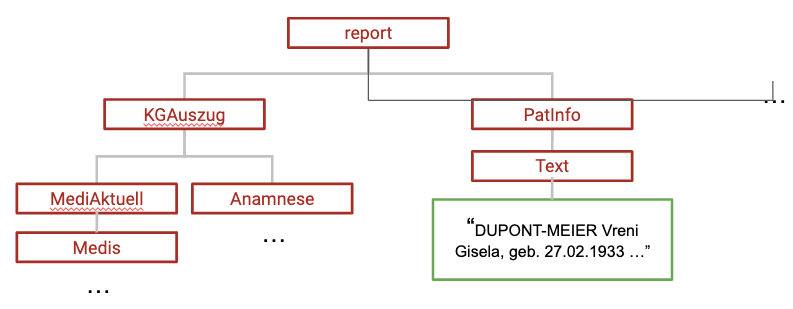
\includegraphics[width=\textwidth]{figs/report_structure.png}
\caption{simple report structure}
\end{figure}

\paragraph{Paths in Field Tree}\label{paths-in-field-tree}

In the various configuration files related to annotations, paths in the
``field tree'' can be used to denote certain parts of the document
(similar to XPath for XML documents).

A \textbf{path} can consist of the following elements: * field name: can
be a
\href{https://docs.oracle.com/javase/8/docs/api/java/util/regex/Pattern.html}{regular
expression accepted by Java} * `/' denoting that the nodes must appear
consecutively, e.g.~\texttt{field\_a/field\_c} matches only
``field\_a/field\_c'' but not ``field\_a/field\_b/field\_c'' . * `//'
denoting that the nodes don't need to be necessarily consecutive, e.g.
\texttt{field\_a/field\_c} would match both ``field\_a/field\_c'' and
``field\_a/field\_b/field\_c''

Note, that paths are case-sensitive.

Examples:
Simple field names which can appear anywhere in the tree: *
\texttt{Id} * \texttt{ID} * some regular expression
\texttt{{[}\textbackslash{}\textbackslash{}p\{IsAlphabetic\}{]}*VisDat}
(``\\p'' is used to match unicode characters). * Field names with some
constraints regarding the parent. For instance, to match \texttt{Text}
fields only when it is a child of \texttt{PatInfo}, you can use
\texttt{//PatInfo//Text}, which would match
e.g.~``/report/PatInfo/some\_element/Text'' * Field constraints
``anchored'' from the top: \texttt{/NOTE} would match a field ``NOTE''
directly under the root of a tree, but not ``/PatientInfo/NOTE''.

\paragraph{Structured Annotations}\label{structured-annotations}

The ``structured annotation step'' allows annotating entire text fields.
For instance, if you know that a certain field contains the name of a
person, then an annotation can be performed at that level.

This step can be parametrized with a configuration file passed in
\texttt{pipeline.structuredFieldMapping} in the pipeline configuration.

Columns in the config file (separated by ``;''): * Path * Annotation
type (e.g.~\texttt{Name}, \texttt{Date} etc) * Features (properties) of
the annotation . Features are separated by ``,'' where key and values
are separated by ``=''

Example: \texttt{//Personalien//Name;\ Name;\ type=patient}

All leaves with \texttt{Name} having \texttt{Personalien} as a parent
somewhere are annotated with \texttt{Name} and having the \texttt{type}
property set to \texttt{patient}.

\paragraph{Field Normalization (Field Annotation
Mapping)}\label{field-normalization-field-annotation-mapping}

Sometimes, we can not blindly annotate an entire field, but need to
apply a JAPE rule on it. For example, signatures could have a structure
like ``ABCD, 20.10.2018'' where ``ABCD'' is the shorthand for a doctor.
Since there are many fields with similar or identical structure, but
different paths the fields can get renamed to a common name. A JAPE rule
processing the pattern would then refer to that common name.

This step can be parametrized with a configuration file passed in
\texttt{pipeline.annotationMapping} in the pipeline configuration.
Columns (separated by ``;''): * Path * New field name

Example: \texttt{//Patient/Alter/Val;\ AgeField}

A field \texttt{Val} with immediate ancestors \texttt{Alter} and
\texttt{Patient} gets named an \texttt{AgeField}. Now a JAPE rule only
working on \texttt{AgeField}s, could for example annotate any number in
there as an age.

\paragraph{Annotation Blacklist}\label{annotation-blacklist}

For some fields we can exclude a priori certain annotations. An example
could be a field containing computer generated identifiers like
\texttt{9b02d92c-c16e-4d71-2019-280237bb8cb5} where a JAPE rule may
erroneously pick up a date (for example ``2019'' in the example). A
blacklisting step would remove such annotations.

This step can be parametrized with a configuration file passed in
\texttt{pipeline.annotationBlacklist} in the pipeline configuration.

Columns (seperated by ``;''): * Path * Comma separated annotation types
which should \emph{not} appear within elements denoted in path

Example: \texttt{//DiagnList//CodeList//Version;\ Date}

The \texttt{Version} field having \texttt{CodeList} and
\texttt{DiagnList} as parents should not contain \texttt{Date}
annotations.

\subsubsection{Context Annotations}\label{context-annotations}

There are some JAPE rules which only get triggered if tokens appear in a
specific language context. This can be useful to disambiguate between
e.g.~surnames and professions or between the profession of a patient vs
the role of staff.

The context can be given by a field (using
\hyperref[field-normalization-field-annotation-mapping]{Annotation Mappings}) or by using
\textbf{context annotations}. They can be added around trigger tokens.
For instance, text in the vicinity of \texttt{Sohn} (son) may contain
his name or information about his profession. Therefore,
\texttt{NameContext} and \texttt{OccupationContext} context annotations
are added to the document, spanning the e.g.~5 tokens before
\texttt{Sohn} and 5 tokens after. Later on, if within these context
annotations e.g.~an isolated first name appears, it can be annotated as
\texttt{Name} since we assume it is a context where names can occur
(otherwise we wouldn't annotate it, as there is not enough evidence).
Context annotations are performed in early stages of the pipeline, s.t.
they can be referred to in JAPE rules later on.

These context triggers can be configured in a config file whose path has
to be provided in \texttt{pipeline.contextTriggerConfig} in the pipeline
configuration.

Columns (separated by ``;''): * Context token (no spaces) * Name of the
context (e.g.~\texttt{NameContext}) * start of the context annotation in
number of tokens before the trigger token * end of the context
annotation in number of tokens after the trigger token

Examples: * \texttt{Sohn;NameContext;5;5} *
\texttt{Partner;OccupationContext;5;5}

\subsection{Test Suite}\label{test-suite}

A small testing framework was developed to test the annotation behavior
of the pipeline in a fast and isolated way. That is, small test cases
can be defined consisting of a phrase and the annotations the pipeline
is expected to produce. This allows for test driven development/tuning
of the annotation pipeline.

\subsubsection{Test Cases Specification}\label{test-cases-specification}

The testcases are described in a textfile. The first line of the text
file contains the annotation types the pipeline is tested against as
well as the context fields. The context fields annotations are used to
test rules based on the document structure. The lists for annotation
types and context fields are seperated by \texttt{;} and the entries in
lists by \texttt{,}.

Then testcases follow, one per line. Manual annotations and fields are
added using XML-tags. Comments using `\#' are allowed either to comment
entire lines are the remainder of a line. Commented parts are ignored.
There may be empty lines for making the file a bit more readable. If new
lines are needed to test a specific situation, this can simply be done
using \texttt{\textbackslash{}n}.

Following an example with 3 test cases:

\begin{verbatim}
Name; FieldWithSignature

Der Patient <Name>Luigi D'Ambrosio</Name> wurde...

<FieldWithSignature>20.01.2018 / <Name>AMUSTER</Name> </FieldWithSignature>
20.01.2018 / AMUSTER # don't expect name annotation in arbitrary fields
\end{verbatim}

In this example, the annotation of \texttt{Name} is tested. The
\texttt{\textless{}Name\textgreater{}} tags are removed before the test
case is passed through the pipeline. Then, the \texttt{Name} annotations
of the pipeline output are checked whether they indeed contain
\texttt{Name} annotations at the same place, and only there. If this is
the case, the test passes, otherwise it fails with an appropriate
message.

The second test case tests a context specific rule, i.e.~the rule is
only applied within fields \texttt{FieldWithSignature} (In the USZ
pipeline, \texttt{FieldWithSignature} annotation is added the annotation
mapping step, see above) The third test case is just to see, if the
previous rule is not triggered outside the required context. Or said
differently, we expect \texttt{AMUSTER} not to be annotated,
i.e.~annotating it would be wrong.

In some existing tests there is also the \texttt{OUTOFVOC} token. It
stands for ``out of vocabulary'' and makes it explicit, that the rule
should rely exclusively on structure, and not be based on entries in the
dictionary.

\subparagraph{Running Tests}\label{running-tests}

A test suite can be run using the \texttt{test} command from the
\texttt{DeidMain} entry point:

\begin{verbatim}
$DEID_CMD test [pipeline configuration file] [testcase directory]
\end{verbatim}

It commands needs a path to a pipeline configuration file
(e.g.~\texttt{configs/kisim-usz/kisim\_usz.conf}) and a directory with
testcases (e.g.~\texttt{configs/kisim-usz/testcases/}). Every
\texttt{*.txt} in that directory is assumed to contain test cases.

The generic rules shipped with the tool are tested using the same
mechanism. They are run as unit tests for the tool itself. The test
cases can be found in the directory
\texttt{deidentifier-pipeline/src/test/resources/pipeline\_testcases}
You normally don't need to modify these tests while tuning the pipeline,
but you may consider them a source of useful examples.


\section{Dictionary and Lexicon Assets}
\subsection{Lexica}\label{lexica}

In GATE, a lexicon (or gazetteer) consists of a text file with one term
per line. A term may contain spaces. The terms are treated as
case-sensitive.

The lexica compiled for the USZ pipeline have many different sources.
Below tables describing the different lexica along with their
provenance. Note, that some lexica cannot be published, as they contain
hospital internal data. Note, that \texttt{ANNIE} refers to a GATE
plugin, \texttt{GeoNames} to the geographical database which can be
found here \texttt{https://www.geonames.org/}.
\newpage

\subsubsection{General}\label{general}
\begin{longtable}[]{@{}
  >{\raggedright\arraybackslash}p{(\columnwidth - 4\tabcolsep) * \real{0.3405}}
  >{\raggedright\arraybackslash}p{(\columnwidth - 4\tabcolsep) * \real{0.2797}}
  >{\raggedright\arraybackslash}p{(\columnwidth - 4\tabcolsep) * \real{0.3797}}@{}}
\toprule\noalign{}
\begin{minipage}[b]{\linewidth}\raggedright
File Name
\end{minipage} & \begin{minipage}[b]{\linewidth}\raggedright
Source
\end{minipage} & \begin{minipage}[b]{\linewidth}\raggedright
Description
\end{minipage} \\
\midrule\noalign{}
\endhead
\bottomrule\noalign{}
\endlastfoot
abbreviations\_stop.lst & ANNIE German & Abbreviations like
\texttt{z.B} \\
general\_wordlist\_with\_uppercased.lst & Aspell dictionary & General
wordlist \\
stop.lst & ANNIE German & Stopwords \\
\end{longtable}

\subsubsection{Locations}\label{locations}
\paragraph{Geographical}\label{geographical}
\begin{longtable}[]{@{}
  >{\raggedright\arraybackslash}p{(\columnwidth - 4\tabcolsep) * \real{0.3064}}
  >{\raggedright\arraybackslash}p{(\columnwidth - 4\tabcolsep) * \real{0.1611}}
  >{\raggedright\arraybackslash}p{(\columnwidth - 4\tabcolsep) * \real{0.5025}}@{}}
\toprule\noalign{}
\begin{minipage}[b]{\linewidth}\raggedright
File Name
\end{minipage} & \begin{minipage}[b]{\linewidth}\raggedright
Source
\end{minipage} & \begin{minipage}[b]{\linewidth}\raggedright
Description
\end{minipage} \\
\midrule\noalign{}
\endhead
\bottomrule\noalign{}
\endlastfoot
additional\_locations.lst & Manually edited & \\
canton\_names.lst & GeoNames and manually added & ``Uri'' \\
cantons\_abbrevs.lst & GeoNames and manually added & ``ZH'', ``BE'' \\
citizenships.lst & Wikipedia and manually added & ``Schweizer'',
``Deutsche'' \\
city.lst & ANNIE & various cities (worldwide) \\
city\_ambiguous\_manual.lst & Manually edited & Cities which typically
have another meaning in the context of medical reports,
e.g.~\texttt{Wangen}, \texttt{Füssen}. No Location annotations are
performed. \\
city\_derived.lst & ANNIE & \\
city\_german.lst & ANNIE & \\
city\_switzerland.lst & Swisstopo Ortschaftenverzeichnis & \\
country.lst & ANNIE & \\
country\_adjectives\_german.lst & Wikipedia and manually added &
``Italienisch'', ``Italienischer'' \\
country\_german.lst & ANNIE & \\
country\_german\_wiki.lst & Wikipedia & Country Names \\
country\_iso\_codes.lst & Manual & \\
country\_manual.lst & Manual & Contains countries not existing
anymore \\
country\_regions\_german\_wiki.lst & Wikipedia & ``Norditalien'' \\
languages\_manual.lst & Manual & \\
larger\_cities.lst & GeoNames & Larger international cities,
``Tripoli'', ``Hannover'' \\
location\_false\_positives.lst & Manual & Typically medical terms
containing location as a part (not annotated) \\
province.lst & ANNIE & \\
regions.lst & Manual & \\
streetnames.lst & Manual & Streets or similar not matching a typical
pattern \\
toponyms\_switzerland.lst & GeoNames & All sorts of topopynms. Extensive
blacklist was needed for ambiguous locations \\
toponyms\_switzerland\_manual.lst & Manual & More Swiss Toponyms \\
\end{longtable}
\newpage

\paragraph{Organisational}\label{organisational}
\begin{longtable}[]{@{}
  >{\raggedright\arraybackslash}p{(\columnwidth - 4\tabcolsep) * \real{0.3483}}
  >{\raggedright\arraybackslash}p{(\columnwidth - 4\tabcolsep) * \real{0.1461}}
  >{\raggedright\arraybackslash}p{(\columnwidth - 4\tabcolsep) * \real{0.5056}}@{}}
\toprule\noalign{}
\begin{minipage}[b]{\linewidth}\raggedright
File Name
\end{minipage} & \begin{minipage}[b]{\linewidth}\raggedright
Source
\end{minipage} & \begin{minipage}[b]{\linewidth}\raggedright
Description
\end{minipage} \\
\midrule\noalign{}
\endhead
\bottomrule\noalign{}
\endlastfoot
buildings\_usz.lst & USZ (KISIM) & Building abbreviations at USZ \\
hospitals.lst & Manual & Hospital names \\
institutions.lst & Manual & Institutions related to USZ \\
organisational\_units\_usz.lst & USZ (KISIM) & Abbreviations of
organisational units \\
related\_organisations\_usz.lst & USZ (KISIM) & Institutions related to
USZ. Internal only. \\
\end{longtable}

\subsubsection{Medical}\label{medical}

Including information about medical terms into the pipeline is mainly to
avoid an annotation on it, typically for surnames.

\begin{longtable}[]{@{}
  >{\raggedright\arraybackslash}p{(\columnwidth - 4\tabcolsep) * \real{0.2745}}
  >{\raggedright\arraybackslash}p{(\columnwidth - 4\tabcolsep) * \real{0.2013}}
  >{\raggedright\arraybackslash}p{(\columnwidth - 4\tabcolsep) * \real{0.5242}}@{}}
\toprule\noalign{}
\begin{minipage}[b]{\linewidth}\raggedright
File Name
\end{minipage} & \begin{minipage}[b]{\linewidth}\raggedright
Source
\end{minipage} & \begin{minipage}[b]{\linewidth}\raggedright
Description
\end{minipage} \\
\midrule\noalign{}
\endhead
\bottomrule\noalign{}
\endlastfoot
drugs\_usz.lst & USZ (KISIM) & \\
medical\_mesh\_terms.lst & MESH 2019 German Translation &
https://www.dimdi.de/dynamic/en/classifications/further-classifications-and-standards/mesh/ \\
medical\_terms\_de.lst & Wikipedia & \\
medical\_terms\_manual.lst & Manual & \\
\end{longtable}

\subsubsection{Occupations}\label{occupations}

Professions and companies a patient might work for.

\begin{longtable}[]{@{}
  >{\raggedright\arraybackslash}p{(\columnwidth - 4\tabcolsep) * \real{0.2500}}
  >{\raggedright\arraybackslash}p{(\columnwidth - 4\tabcolsep) * \real{0.1100}}
  >{\raggedright\arraybackslash}p{(\columnwidth - 4\tabcolsep) * \real{0.6400}}@{}}
\toprule\noalign{}
\begin{minipage}[b]{\linewidth}\raggedright
File Name
\end{minipage} & \begin{minipage}[b]{\linewidth}\raggedright
Source
\end{minipage} & \begin{minipage}[b]{\linewidth}\raggedright
Description
\end{minipage} \\
\midrule\noalign{}
\endhead
\bottomrule\noalign{}
\endlastfoot
company\_list\_ch.lst & Wikipedia & \\
generic\_occupations.lst & Manual & More for testing purposes \\
occupations\_usz.lst & USZ Kisim & Processed list of professions entered
in KISIM. Internal only. \\
\end{longtable}

\subsubsection{Person Names}\label{person-names}

A few lexica are partitioned into two parts with ``frequent'' and
``seldom'' names. The distinction is used by some rules as indication
whether a token might likely be a name or not.

\begin{longtable}[]{@{}
  >{\raggedright\arraybackslash}p{(\columnwidth - 4\tabcolsep) * \real{0.3274}}
  >{\raggedright\arraybackslash}p{(\columnwidth - 4\tabcolsep) * \real{0.4867}}
  >{\raggedright\arraybackslash}p{(\columnwidth - 4\tabcolsep) * \real{0.1858}}@{}}
\toprule\noalign{}
\begin{minipage}[b]{\linewidth}\raggedright
File Name
\end{minipage} & \begin{minipage}[b]{\linewidth}\raggedright
Source
\end{minipage} & \begin{minipage}[b]{\linewidth}\raggedright
Description
\end{minipage} \\
\midrule\noalign{}
\endhead
\bottomrule\noalign{}
\endlastfoot
firstnames\_switzerland\_frequent.lst & Bundesamt für Statistik:
Vornamen in der Schweiz 2017 & \\
firstnames\_switzerland\_seldom.lst & Bundesamt für Statistik: Vornamen
in der Schweiz 2017 & \\
firstnames\_usz\_frequent.lst & USZ (KISIM) & \\
name\_false\_positives.lst & Manual & Often medical terms \\
surnames\_usz\_frequent.lst & USZ (KISIM) & \\
firstnames\_usz\_seldom.lst & USZ (KISIM) & Internal only \\
surnames\_staff\_usz.lst & USZ (KISIM) & Internal only \\
surnames\_usz\_seldom.lst & USZ (KISIM) & Internal only \\
\end{longtable}

\subsubsection{Suffix Lists}\label{suffix-lists}

Instead of using lexica annotating terms 1:1 in the text, a part of the
pipeline annotates tokens based on suffixes. This is useful for missing
terms in the other dictionaries. For example \texttt{Nasenerkrankung}
would still be recognized as medical term, even though it might not be
in any medical dictionary.

\begin{longtable}[]{@{}lll@{}}
\toprule\noalign{}
File Name & Source & Description \\
\midrule\noalign{}
\endhead
\bottomrule\noalign{}
\endlastfoot
medical\_suffixes.lst & Manual &
\texttt{erkrankung},\texttt{geräusch} \\
surname\_suffixes.lst & Manual & \texttt{mann},\texttt{oulos} \\
\end{longtable}


\section{Software Development and Updates}
%\section{Development}\label{development}

For more details on the \href{code_overview.md}{code structure here}

\subsection{Releases}\label{releases}

Releases can be done via github actions and the built jar and users can
download it on the
\href{https://github.com/ratschlab/medical-reports-deidentification/releases}{github
release page}

\begin{enumerate}
\def\labelenumi{\arabic{enumi}.}
\tightlist
\item
  Adapt the version in the \texttt{\textless{}version\textgreater{}}
  section of \href{https://github.com/ratschlab/medical-reports-deidentification/blob/main/deidentifier-pipeline/pom.xml}{maven config}
\item
  merge this change into main
\item
  create a tag locally on your computer using
  \texttt{git\ tag\ v{[}version{]}}, e.g.~\texttt{git\ tag\ v1.0.0}
\item
  push tag using \texttt{git\ push\ origin\ v1.0.0} (adapt to the
  version)
\item
  If the github actions workflow ran successfully, you can edit the
  release as necessary on the
  \href{https://github.com/ratschlab/medical-reports-deidentification/releases}{github
  release page} and switch it from Pre-release to release (remove the
  flag \texttt{This\ is\ a\ pre-release})
\end{enumerate}

Note, that there is a danger that the version in \texttt{pom.xml} and in
the git tag don't match. This could/should be streamlined in the future.


\section{Data Processing and Workflow Structuring}
\subsection{Diagnosis Extraction
Pipeline}\label{diagnosis-extraction-pipeline}

This document briefly describes a pipeline to extract diagnosis out of a
medical report along with a (rough) estimate on its reliability
(confirmed, suspected, excluded).

\subsubsection{Approach}\label{approach}

The current implementation is mainly based on keyword matching and is
hence very basic. An initial evaluation shows that the diagnosis are
extracted well, however, the reliability of the diagnosis are not
detected very reliably as the language around suspected or excluded
cases can be involved. Because of way the pipeline is currently
implemented, there is a bias towards `confirmed' diagnosis, i.e the
pipeline may label a diagnosis as \texttt{confirmed} whereas the actual
diagnosis was merely a suspection or even an exclusion.

\subsubsection{Pipeline Overview}\label{pipeline-overview}

The pipeline is based on the same framework as the deidentification
pipeline and hence shares many commonalities.

The input is the same as for the \texttt{annotation} tool i.e.~reports
out of KISIM either directly from a database or already imported as GATE
documents.

The pipeline generates for every diagnosis the following output:

\begin{itemize}
\tightlist
\item
  document ID/report ID
\item
  annotation text found related to diagnosis (mainly for debugging)
\item
  code (ICD-10)
\item
  reliability of diagnosis: confirmed, suspected, excluded
\end{itemize}

Note, that per report several diagnosis may be extracted. Furthermore,
the reliabilities may be conflicting, that is, in a report there may be
the same diagnosis twice with different reliabilities. Depending on the
use case, the downstream system need to resolve this ``conflict''.

These fields can be written back to a database table and/or written to a
text file for further analysis in pandas/excel.

\subsubsection{Configuration}\label{structuring-configuration}

\paragraph{Database Configuraiton}\label{database-configuraiton}

The configuration related for reading and writing into the database are
the same as with the deidentification pipeline. There are just a few
more configuration keys related to the naming of the fields generated by
the diagnosis extraction pipeline:

\begin{verbatim}
annotationtext_field_name=annotationtext
reliability_field_name=reliability
code_field_name=code
\end{verbatim}

These properties can be changed to match the destination table schema.
The same keys should then be used in the \texttt{dest\_columns}
property.

For example:

\begin{verbatim}
dest_columns=reportnr,fcode,dat,fallnr,annotationtext,code,reliability
\end{verbatim}

\paragraph{Pipeline Configuration}\label{pipeline-structuring-configuration}

Many aspects of the pipeline can be tweaked by editing text files.

\subparagraph{Keywords Configuration}\label{keywords-configuration}

For every ICD-10 code to be extracted there needs to be a few
keywords/names for the condition. The keyword configuration file is a
text file where a row corresponds to one ICD-10 code. The fields are
separated by \texttt{;} and constituting the following:

\begin{itemize}
\tightlist
\item
  ICD-10 code, for example \texttt{G35};
\item
  keywords separated by \texttt{,}, for example
  \texttt{Multiple\ Sklerosis,Encephalitis\ disseminata}
\item
  blacklist paths: paths in the document structure which should not be
  considered to search for the keyword:
  e.g.~\texttt{Header,Fragestellung} (see also
  \texttt{Paths\ in\ Field\ Tree} in \texttt{components.md})
\end{itemize}

\subparagraph{Reliability Context
Configuration}\label{reliability-context-configuration}

In order to assess the reliability of a diagnosis the `reliability
context' of a diagnosis is determined. This is done in a very crude way
by looking for keywords within the neighborhood of a diagnosis keyword.
For instance \texttt{ausgeschlossen} somewhere close after a diagnosis
term like \texttt{Multiple\ Sklerose} could mean that the diagnosis is
excluded.

These keywords can be configured the in reliability context
configuration file. This is a textfile with one keyword a line, where
the fields are separated by \texttt{;}. The fields are as follows

\begin{itemize}
\tightlist
\item
  context keyword, e.g.~\texttt{ausgeschlossen}
\item
  context name: \texttt{ExclusionContext} or \texttt{SuspectionContext}
\item
  left extend: number of tokens from the context keyword to the left,
  the context is valid
\item
  right extend: number of tokens from the context keyword to the right
\end{itemize}

\subsubsection{Invocation}\label{invocation}

The entry point of the pipeline is the
\texttt{org.ratschlab.structuring.DiagnosisExtractionCmd} class. It has
the following usage (note, that currently not all options are
implemented).

\begin{verbatim}
 Usage: <main class> [--json-input] [--xml-input]
                     [--doc-id-filter=<docIdFilterPath>]
                     [--doc-type-filter=<docTypeFilterPath>]
                     [--max-docs=<maxDocs>]
                     [--output-corpus-dir=<outputCorpusDir>]
                     [--skip-docs=<skipDocs>] -c=<pipelineConfigFile>
                     [-d=<databaseConfigPath>] [-i=<corpusInputDir>]
                     [-o=<outputFile>] [-t=<threads>]
       --doc-id-filter=<docIdFilterPath>
                              Path to file id list to consider
       --doc-type-filter=<docTypeFilterPath>
                              Path to file type list to consider
       --json-input           Assumes input dir consists of json files, one per
                                report (testing purposes)
       --max-docs=<maxDocs>   Maximum number of docs to process
       --output-corpus-dir=<outputCorpusDir>
                              Output GATE Corpus Dir
       --skip-docs=<skipDocs> Skipping number of docs (useful to just work on a slice
                                of the corpus)
       --xml-input            Assumes input dir consists of xml files, one per report
                                (testing purposes)
   -c=<pipelineConfigFile>    Config file
   -d=<databaseConfigPath>    DB config path
   -i=<corpusInputDir>        Input corpus dir
   -o=<outputFile>            Output Txt File
   -t=<threads>               Number of threads
\end{verbatim}

\subsubsection{Pipeline Description}\label{pipeline-description}

The pipeline executes the following steps for every document:

\begin{enumerate}
\def\labelenumi{\arabic{enumi}.}
\tightlist
\item
  tokenization of the import report
\item
  diagnosis keywords are annotated
\item
  reliability contexts are annotated
\item
  JAPE rules are run to

  \begin{itemize}
  \tightlist
  \item
    determine the reliability of a diagnosis by either checking whether
    it is within some reliability context or whether it matches a
    certain language pattern (e.g.~\texttt{Verdacht\ auf} \ldots)
  \item
    Removing some false positives like
    \texttt{some\_diagnosis\ Sprechstunde} or
    \texttt{some\_diagnosis\ Abklaerung}
  \end{itemize}
\item
  Consolidate diagnosis anntoations: * adding \texttt{confirmed}
  reliability as default, if no other reliability could be determined *
  removing duplicates
\item
  Writing to file and/or database
\end{enumerate}


\section{Annotation Rules and Optimization Strategies}
\subsection{Rules Guide and Tuning}\label{rules-guide-and-tuning}

This section describes how the rules are set up as well as their current
limitations. Also, some typical tuning scenarios are described. We
assume the reader is familiar with the \href{components.md}{annotation
pipeline components}.

\subsubsection{General Considerations}\label{general-considerations}

In general, we need to balance between annotating as many relevant
tokens as possible not annotating ``too much''. That is, we'd like to
have a high recall (few false negatives), but still maintain a
reasonable precision (few false positives), otherwise the data quality
of downstream applications may suffer.

Typically, annotations carry attributes to be able to trace back to the
rule generating it. This is very useful for debugging.

There are also a few ``negative'' rules, i.e.~rules which ``consume''
tokens but don't trigger annotations. This is typically to avoid false
positives. An example are citations like \texttt{Meier\ et\ al.}, where
\texttt{Meier} should not be annotated as surname to be deidentified,
since it is a citation.

\subsubsection{Date Annotation}\label{date-annotation}

Dates are a fairly closed category, that is, as long as most patterns
are captured in the rules how dates can be written, the annotation works
well.

There is one slightly more challenging pattern where the year as well as
the last \texttt{.} is missing like in \texttt{10.1} meaning 10th of
January. Some care needs to be taken to correctly distinguish such dates
from decimal numbers (which are e.g. followed by some unit).

Remaining issues are mainly due to misspellings of dates such as
\texttt{16.11.2918} or \texttt{21.111.2018} or \texttt{20.102015}.
Although to a human reader it is clear what date is actually meant, it
is not straightforward to capture these in patterns. This could be
addressed in future extensions.

\paragraph{Information Extraction for
Dates}\label{information-extraction-for-dates}

Additionally to recognizing dates in text, the annotation pipeline also
attempts to infer the structure of dates. This includes determining the
date format, e.g.~``dd.MM.yyyy'' as well as to extract day, month and
year components. This is helpful later on, when substitution is done
with the \texttt{ReplacementTags} strategy.

The formats extracted are compatible with the
\href{https://docs.oracle.com/javase/8/docs/api/java/text/SimpleDateFormat.html}{SimpleDataFormat}
in Java. Note, that the information extraction is not guaranteed to
succeed, i.e.~fields may be missing/empty.

\subsubsection{Name Annotation}\label{name-annotation}

Name annotations are driven by triggers such as titles like \texttt{Dr.}
or names from lexika. That is, tokens like \texttt{Dr.}, \texttt{Frau},
\texttt{Prof} etc are most of the time followed by a name. Some rules
exploit this fact.

Names not preceded by such trigger tokens are recognized using lexica.
Note, that blindly annotating tokens appearing in name lexica will lead
to many false positives, e.g.~\texttt{Iris} may be annotated as name
although the part of the eye is meant. Hence, some more ``evidence'' is
needed, that a name candidate is indeed a name. This includes: * token
is followed/preceded by another token appearing in a name lexicon *
token is a frequent name and the token doesn't appear in any medical or
general lexica

This approach requires lexica of good quality, i.e.~they should be
reasonably complete and not contain tokens which are not actually names
(may be problematic if lexica directly compiled from a hospital database
system)

Special care is also taken to not annotate citations such as
\texttt{Meier\ et\ al.}

\paragraph{Shorthands/Abbreviations}\label{shorthandsabbreviations}

Shorthands or abbreviations of hospital staff also fall in the name
category. At USZ staff shorthands are typically 5 characters long
(although the length ranges from 3 to 8 characters) and most of the time
spelled in upper case, such as \texttt{ABCDE}.

Since shorter abbreviations of 3 or 4 characters may also simply be a
(medical) acronym, the annotation of such strings is only triggered in
certain fields. Some report specific rules were needed for some report
types where the shorthands are spelled in small case.

\paragraph{Information Extraction for
Names}\label{information-extraction-for-names}

Similar to the \texttt{Date} annotation, the structure of a
\texttt{Name} annotation is also extracted by the pipeline, e.g.~the
firstname and lastname. If a salutation could be recognized, it is also
included (this can be used during a substitution procedure to determine
the gender of the involved name).

The following fields are extracted:

\begin{longtable}[]{@{}
  >{\raggedright\arraybackslash}p{(\columnwidth - 4\tabcolsep) * \real{0.3824}}
  >{\centering\arraybackslash}p{(\columnwidth - 4\tabcolsep) * \real{0.4412}}
  >{\raggedleft\arraybackslash}p{(\columnwidth - 4\tabcolsep) * \real{0.1765}}@{}}
\toprule\noalign{}
\begin{minipage}[b]{\linewidth}\raggedright
Field
\end{minipage} & \begin{minipage}[b]{\linewidth}\centering
Example
\end{minipage} & \begin{minipage}[b]{\linewidth}\raggedleft
Description
\end{minipage} \\
\midrule\noalign{}
\endhead
\bottomrule\noalign{}
\endlastfoot
firstname & Hans & \\
lastname & Meier-Müller & \\
signature & ABCDE & internal abbreviation/shorthand \\
salutation & Frau Dr. & complete salutation (usually preceding an
annotation) \\
format & ff ll & structure of name \\
\end{longtable}

The format field is composed of following tokens:

\begin{longtable}[]{@{}lc@{}}
\toprule\noalign{}
Letters & Meaning \\
\midrule\noalign{}
\endhead
\bottomrule\noalign{}
\endlastfoot
f & firstname short (typically 1 letter) \\
ff & full firstname \\
ll & lastname \\
LL & lastname all upper case: \texttt{MEIER} \\
s & signature \\
S & signature all upper case \\
\end{longtable}

Note, that fields may be empty. Furthermore, if an annotation can be
called by various rules, the extracted information can be contradictory
(contradictory information is separated by \texttt{,}). For instance,
the text \texttt{Peter\ Simon} may be called by 2 rules, one for double
lastnames and one for double first names leading to contradictory values
for \texttt{format} (and also \texttt{firstname} and \texttt{lastname}).
These conflicts are currently not resolved and need to be handled by the
downstream pipeline.

\subsubsection{Location Annotation}\label{location-annotation}

This is a fairly broad category encompassing physical locations such as
places and countries (by extension also languages) as well as
organizations such as hospitals, departments within hospitals, medical
practices etc.

\texttt{Location} annotations heavily depend on good lexica. There are a
few rules to recognize street names and zip codes. Also many health care
organizations can be recognized by certain triggers like
\texttt{Spital}, \texttt{Altersheim} etc. These triggers are also
important to recognize organizations which may be in some lexica, but
are referred to differently by the medical staff
(e.g.~\texttt{Altersheim\ XY} instead of the official
\texttt{Pflegezentrum\ XY}).

Challenges arise with ambiguous locations such as \texttt{Wangen} (place
and ``cheeks'') as well as with misspellings \texttt{Grüningen} vs
\texttt{Grünigen}, \texttt{*thal} vs \texttt{*tal}.

\subsubsection{Occupation Annotation}\label{occupation-annotation}

Both patterns and lexica are important to recognize occupations.
Similarly with names, we cannot blindly annotate tokens which appear in
a occupation dictionary, since the token may designate for example a
surname or the profession or role of somebody involved with the patient,
but not the patient him/herself (e.g.~\texttt{beim\ Augenarzt},
\texttt{Polizist}).

\subsubsection{Tuning Guidelines}\label{tuning-guidelines}

In case a token should have been annotated by the pipeline and it
wasn't, the following steps could be taken: * first (!) add a test case
to the test suite. Perhaps don't take the original data for privacy
reasons but slightly alter it to reflect the situation. Verify the test
case fails (\texttt{make\ test}). * if appropriate, add more tokens to
corresponding lexicon * if appropriate, tweak existing rule or add a new
rule * verify the test(s) passes now.

The same procedure can roughly be followed if a token was wrongly
annotated. In this case, perhaps entries need to be removed from a
lexicon. Or in some added to a ``false positive'' or ``ambiguous''
dictionary. Refer to the \href{lexica.md}{lexica overview} to pick an
appropriate lexicon to edit.

When editing lexica try to limit the editing to lexica marked as
``manual'' in \href{lexica.md}{lexica overview}. This way, if other
types of lexica get regenerated by a script, your changes don't get
overwritten.


\section{Guidelines for System Tuning}
\subsection{Tuning Tutorial}\label{tuning-tutorial}

Here few hands-on ``exercises'' on how to tune the pipeline on a heavily
simplified version of the USZ deidentification pipeline. The goal is to
get familiar with the various components in a simplified setting without
being overwhelmed by all the details of a full-fledged pipeline.

\subsubsection{Setup}\label{setup}

To test whether modification of the pipeline lead to the desired
behavior, we are going to use the testing framework included in the
deidentification tool. Tests for many of the exercises below are already
prepared in the \texttt{configs/tutorial/testcases}, they just need to
be uncommented (i.e.~removing the \texttt{\#})

The test suite can be run using the following command:

\begin{verbatim}
java -jar [path to jar file] test [pipeline config file] [test cases directory]
\end{verbatim}

where \texttt{{[}path\ to\ jar\ file{]}} should point to a current
\texttt{jar} file of the pipeline (typically
\texttt{deidentifier-*.jar}), \texttt{{[}pipeline\ config\ file{]}} to
some path ending with \texttt{configs/tutorial/tutorial.conf} and
\texttt{{[}test\ cases\ directory{]}} a path ending on
\texttt{configs/tutorial/testcases}. Tip: put the resulting long command
into a \texttt{.bat} or \texttt{.sh} file which you then execute.

When running the test suite, if everything goes well, you should see
lines containing \texttt{Reading\ testcases\ from} at the end. If a
testcase should fail, a clear error message is displayed with some more
details what went wrong.

\subsubsection{Exercices}\label{exercices}

\paragraph{Add test case for dates}\label{add-test-case-for-dates}

In the file \texttt{date.txt} there is already one test case defined to
check whether a date is indeed recognized. Uncomment that line and run
the test suite. You should see something like

\begin{verbatim}
2019-12-06 13:27:40.891 INFO  org.ratschlab.deidentifier.pipelines.testing.PipelineTestSuite - Reading testcases from configs/tutorial/testcases/date.txt
2019-12-06 13:27:40.895 INFO  org.ratschlab.deidentifier.pipelines.testing.PipelineTester - Running test suite with 1 test cases
\end{verbatim}

On a new line add another date without the
\texttt{\textless{}Date\textgreater{}} tags. Run the test suite again
and see how it fails. Add the tags, run again and this time the suite
should pass.

\paragraph{Add missing location}\label{add-missing-location}

The location \texttt{Oberikon} is not recognized in a document. Add a
test case for it in the \texttt{locations.txt} file and run the test
suite. It should fail on that test. Then, add the place to some
appropriate lexikon (e.g.~in the already existing
\texttt{locations/additional\_locations.lst}). After that, the test
suite

\paragraph{Internal phone number
format}\label{internal-phone-number-format}

Assume internal phone numbers consist of two blocks of 3 digits, e.g.:
\texttt{123\ 456}. Write a JAPE rule which recognizes these numbers.
There is already some test case in \texttt{contact.txt}

Hints: * add the rule in \texttt{specific-rules/contacts.jape}. There is
already some rule recognizing some Swiss phone numbers (copied from the
generic JAPE rule set). * See
https://gate.ac.uk/sale/thakker-jape-tutorial/GATE\%20JAPE\%20manual.pdf
if you'd like to know more about how JAPE rules work. * In practice, you
would probably add a ``trigger'' on the left side, i.e.~fire the rule
only if the two blocks are preceded by a ``Tel'' token.


\section{Performance Evaluation and Metrics}
\subsection{Evaluation Guide}\label{evaluation-guide}

We sketch how to evaluate the performance of the pipeline on your
reports.

\subsubsection{Create Goldstandard Set}\label{create-goldstandard-set}

One approach is to annotate relevant reports using the existing pipeline
(using the \texttt{annotate} command) and let experts check/complement
the resulting annotations. Alternatively, you can simply convert the
reports to the GATE internal format using the \texttt{import} command.
In this case, the annotator would have to create all annotations
manually, which can be very tedious.

\paragraph{Annotation Guide}\label{annotation-guide}

First, install \href{https://gate.ac.uk/download/}{GATE Developer}.

If you haven't already, load the \texttt{Schema\ Annotation\ Editor} via
\texttt{File} -\textgreater{} \texttt{Manage\ CREOLE\ Plugins}. Tick
\texttt{Load\ now} and \texttt{Load\ always} next to
\texttt{Schema\ Annotation\ Editor}. Restart GATE

Load a schema into GATE: right click on \texttt{Language\ Resources} in
the explorer view, choose \texttt{New} -\textgreater{}
\texttt{Annotation\ Schema}. Click on the briefcase symbol on look for
the
\href{https://github.com/ratschlab/medical-reports-deidentification/blob/main/deidentifier-pipeline/src/main/resources/schemas/master.xml}{master.xml}
file on your filesytem . Open a GATE document, activate
\texttt{Annotation\ Sets} view and select the phi-annotations-manual
annotation set on the right.

Make sure, schemas are loaded in GATE before you open a corpus to
annotate. Load the corpus via \texttt{File} -\textgreater{}
\texttt{Datastores} -\textgreater{} \texttt{Open\ Datastore}. Load
document and add necessary annotations by marking some tokens and
pressing \texttt{Ctrl+E} When creating a new annotation, make sure
\texttt{phi-annotations} is selected on the right hand side. Regularly
do Right-click on document then \texttt{Save\ to\ its\ datastore} (not
done automatically!)

Also make sure reports are read-only to not accidentally edit the
document:

\begin{figure}
\centering
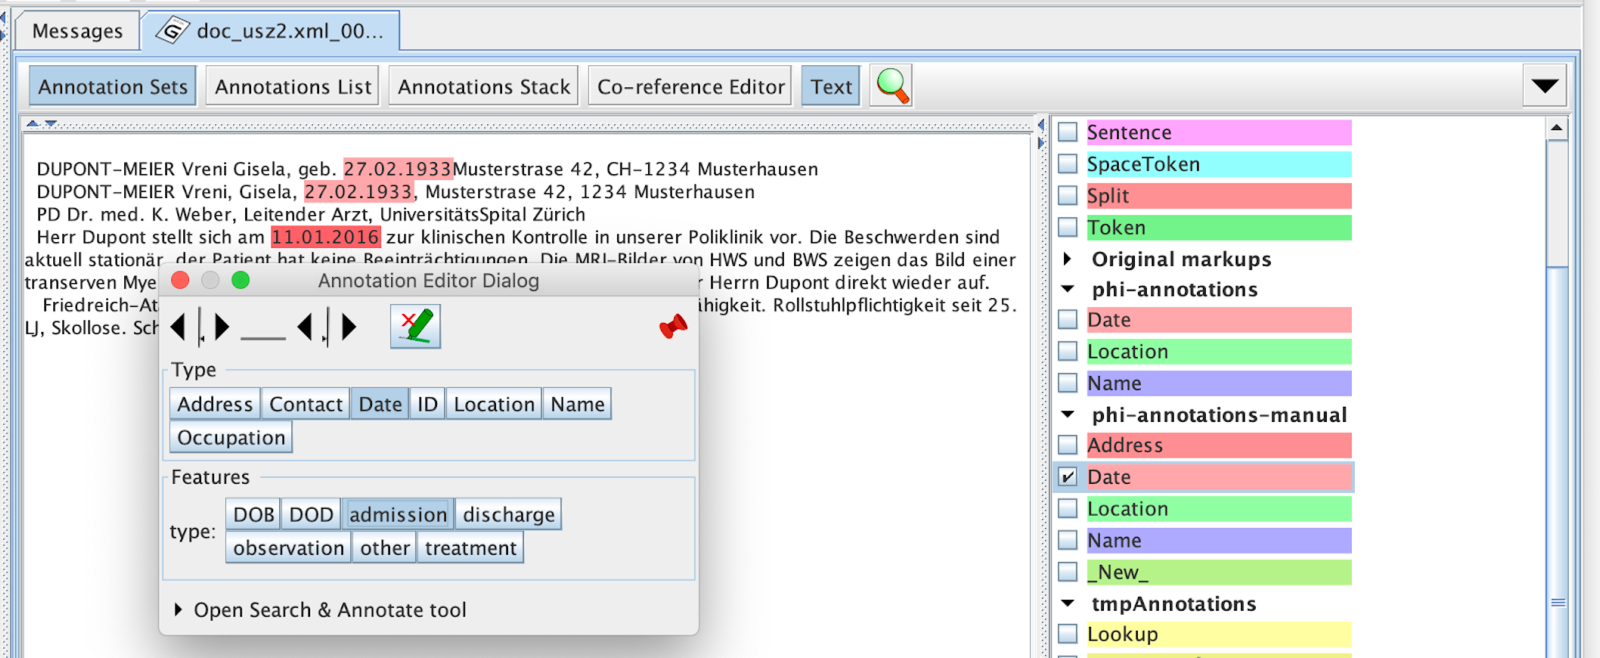
\includegraphics[width=\textwidth]{figs/annotation_dialog.png}
\caption{Annotation View}
\end{figure}

\subsubsection{Evaluate with Respect to Goldstandard
Set}\label{evaluate-with-respect-to-goldstandard-set}

To compare the pipeline output to the goldstandard corpus, annotate the
same reports using the \texttt{annotate} comman, but this time add the
\texttt{-m} option with the path to the goldstandard corpus (\texttt{m}
for ``marked''). You can also add the option
\texttt{-\/-diagnostics-dir} with path where diagnostics information
should be output. It will contain a performance summary in
\texttt{corpus-stats.html} as well detailed output for every report.

\paragraph{Analyse Results in More
Details}\label{analyse-results-in-more-details}

With the \texttt{-\/-diagnostics-dir} option, various ``features'' of
every token are extracted and stored in json files in the
\texttt{ml-features.json}. These features include the annotations of the
pipeline and the rule generating the annotation as well as the
annotations from the goldstandard (if available). They also include in
what lexica a token was found, in what field the token appeared, the
position within the sentence.

These json file(s) can be converted to parquet using a
\href{https://github.com/ratschlab/medical-reports-deidentification/blob/main/scripts/convert_ml_features_to_parquet.py}{python script} and
then explored in a jupyter notebook. This is very helpful to get an
overview over problems in one or several corpora.


\section{Case Study: Pipeline Performance on Report from University Hospital Zurich}
\subsection{Pipeline Evaluation}\label{pipeline-evaluation}

\subsubsection{Method and Corpus}\label{method-and-corpus}

400 reports from the University Hospital Zurich were picked at random
across around 30 document types (mainly discharge reports) giving rise
to around 2.7 Mio tokens. These reports then got annotated using a
prelimninary version of the pipeline. A medical student then went
through these annotations in GATE Developer and complemented/corrected
the existing ones. In a last step, the annotations got checked by a
member of the USZ staff. Then, the annotations of the mature version of
the pipeline was compared to the verified annotations (``goldstandard'')
and evaluated.

The corpus was split into two parts with 200 reports each. The first
part was heavily used for development and tuning (``training set'')
whereas the second was only used for evaluation (``validation set''). No
evaluation on a strictly unseen test set was performed.

A bit more details can be found in Section~\ref{evaluation-guide}.

\subsubsection{Results}\label{results}

The following tables contain Precision/Recall by annotation types
comparing the pipeline output with the annotations in the goldstandard.
The \texttt{Recall} and \texttt{Precision} columns refer to exact
matches of annotations, the columns \texttt{Recall\ Lenient} and
\texttt{Precision\ Lenient} also include partial matches, for instance,
for the name \texttt{Hanna\ Meier\ Huber}, the pipeline only annotates
\texttt{Hanna\ Meier}.

\paragraph{Entire Goldstandard Corpus (Parts I +
II):}\label{entire-goldstandard-corpus-parts-i-ii}

\begin{longtable}[]{@{}llllll@{}}
\toprule\noalign{}
Type & Matches & Recall & Recall Lenient & Precision & Precision
Lenient \\
\midrule\noalign{}
\endhead
\bottomrule\noalign{}
\endlastfoot
Age & 716 & 94.584 & 94.584 & 95.086 & 95.086 \\
Contact & 4805 & 99.154 & 99.505 & 99.154 & 99.505 \\
Date & 47223 & 99.145 & 99.397 & 98.574 & 98.825 \\
ID & 187 & 79.915 & 85.897 & 3.166 & 3.403 \\
Location & 31427 & 85.300 & 91.415 & 84.309 & 90.353 \\
Name & 17422 & 98.787 & 99.484 & 94.561 & 95.229 \\
Occupation & 290 & 55.238 & 63.619 & 60.291 & 69.439 \\
\end{longtable}

\paragraph{Goldstandard Part I}\label{goldstandard-part-i}

\begin{longtable}[]{@{}llllll@{}}
\toprule\noalign{}
Type & Matches & Recall & Recall Lenient & Precision & Precision
Lenient \\
\midrule\noalign{}
\endhead
\bottomrule\noalign{}
\endlastfoot
Age & 361 & 96.524 & 96.524 & 93.282 & 93.282 \\
Contact & 2384 & 99.375 & 99.625 & 98.962 & 99.211 \\
Date & 24686 & 99.252 & 99.481 & 98.673 & 98.901 \\
ID & 82 & 80.392 & 87.255 & 2.495 & 2.708 \\
Location & 16220 & 87.576 & 93.391 & 84.020 & 89.599 \\
Name & 9195 & 98.712 & 99.377 & 93.445 & 94.075 \\
Occupation & 157 & 60.153 & 68.966 & 62.800 & 72.000 \\
\end{longtable}

\paragraph{Goldstandard Part II}\label{goldstandard-part-ii}

\begin{longtable}[]{@{}llllll@{}}
\toprule\noalign{}
Type & Matches & Recall & Recall Lenient & Precision & Precision
Lenient \\
\midrule\noalign{}
\endhead
\bottomrule\noalign{}
\endlastfoot
Age & 355 & 92.689 & 92.689 & 96.995 & 96.995 \\
Contact & 2421 & 98.937 & 99.387 & 99.343 & 99.795 \\
Date & 22537 & 99.029 & 99.306 & 98.466 & 98.742 \\
ID & 105 & 79.545 & 84.848 & 4.009 & 4.276 \\
Location & 15207 & 82.999 & 89.417 & 84.620 & 91.164 \\
Name & 8227 & 98.870 & 99.603 & 95.841 & 96.552 \\
Occupation & 133 & 50.379 & 58.333 & 57.576 & 66.667 \\
\end{longtable}

\subsubsection{Annotation Issues
Observed}\label{annotation-issues-observed}

\paragraph{Age}\label{age}

Issues with more complex sentence structures, such as

\begin{itemize}
\tightlist
\item
  \texttt{Brüder\ verstorben\ mit\ 77,\ 71\ und\ 78\ Jahren}
\item
  \texttt{Sie\ sei\ eigentlich\ 49\ und\ nicht\ 42\ Jahre\ alt}
\end{itemize}

\paragraph{Contact}\label{contact}

Some hospital internal phone numbers were not recognized.

\paragraph{Date}\label{date}

Some scores are erroneously recognized as dates.

\begin{itemize}
\tightlist
\item
  \texttt{Nutritional\ Assessment:\ 7/15,\ Faszikulationen\ an\ 10/10\ Stellen}
\item
  \texttt{Beginn:\ 1.2,\ Albuminquotient\ 13.4}
\end{itemize}

\paragraph{ID}\label{id}

The extremely low precision comes from the fact, that what is considered
as IDs was changed. That is, some entities now annotated by the pipeline
are not annotated in the goldstandard. For the recall, some model
numbers were erroneously annotated in the gold standard

\paragraph{Location}\label{location}

The somewhat medium performance in the location category originates in
the broad definition including place names and terms referring to names
of organisations or organisational units. It is also not always clear
whether terms like \texttt{Physiotherapie}, \texttt{Unfallchirurgie},
\texttt{Innere\ Medizin} and the like are part of an organization name
or are just generic medical terms not carrying any identifying meaning.
This sort of ambiguous case make up the largest part.

A more detailed look reveals, that the pipeline missed very few patient
related location information, that is a 7 locations outside Switzerland
in Goldstandard Part I. About 10 organisations were missed.

\paragraph{Name}\label{name}

Great care was taken to not miss names of patients or staff, i.e.~the
pipeline is tuned for a high recall. The comparatively low precision is
due to the fact, that some staff abbreviations were not annotated in the
goldstandard corpus. Another problem are that medical terms like
\texttt{M.\ Scheuermann}, \texttt{Spina}, \texttt{Carina},
\texttt{Karina}, \texttt{B.\ Fieber} get annotated as names.

\paragraph{Occupation}\label{occupation}

This is a difficult category to annotate, since the way professions or
occupations can be expressed are quite variable. They typically occur
in certain fields related to anamnesis. These can be excluded using
the \texttt{-\/-fields-blacklist} option in the substitute command
(Section~\ref{substitution-policies}) if the risk is too high.


\section{Discussion and Summary}
%\section{Discussion and Summary}

This document has detailed the development and deployment of a
sophisticated de-identification tool for clinical reports, designed to
ensure privacy and compliance with health data regulations. Through
rigorous testing, including a focused case study at the University
Hospital Zurich, the tool has demonstrated high effectiveness in
recognizing and anonymizing personal health information
(PHI). Notably, the tool achieves high precision and recall across
various data types, with particularly robust performance in handling
names and dates, which are common identifiers in clinical data.

Challenges remain in accurately identifying and processing less
structured data and nuanced PHI elements, which sometimes lead to
inconsistencies, particularly in free-text fields. Future improvements
will focus on enhancing the tool's machine learning models to better
understand contextual nuances and reduce false positives, thereby
increasing the reliability of the de-identification process.

Overall, the tool stands as a critical asset in the realm of medical
data processing, offering robust privacy safeguards without
compromising the utility of the data for research and clinical review.

\section{Discussion and Summary}

This document has detailed the development and deployment of a
sophisticated de-identification tool for clinical reports, designed to
ensure privacy and compliance with health data regulations. Through
rigorous testing, including a focused case study at the University
Hospital Zurich, the tool has demonstrated high effectiveness in
recognizing and anonymizing personal health information
(PHI).

{\bf Notably, the tool achieves over 99\% recall in identifying and
  anonymizing 'Contact', 'Date', and 'Name' entities, and
  approximately 95\% for 'Age', with 'Location' entities recognized
  with about 91\% recall.} These results underscore the tool's robust
capability to safeguard sensitive information.  Challenges remain in
the lower recall rates for 'ID' and 'Occupation', which are 85\% and
64\%, respectively. However, these entities are considered less
critical from a privacy standpoint as 'ID' numbers appear infrequently
and occupations are generally not too specific. {\bf If a recall
  threshold of at least 90\% is set as a benchmark for privacy
  concerns, this tool reliably removes critical PHI categories such as
  Age, Contact, Date, Location, and Names.}

Future improvements will focus on enhancing the tool's machine
learning models to better understand contextual nuances and reduce
false positives, thereby increasing the reliability of the
de-identification process. This ongoing enhancement will ensure that
the tool not only meets the regulatory requirements but also adapts
efficiently to varied data formats and clinical environments,
maintaining high standards of patient privacy without compromising the
utility of the data for research and clinical review.



\end{document}
